\section{Coding Inefficiencies}
\label{identification}

Inefficiency removal is a two stage iterative process, where bottlenecks are identified and later removed. First, the application is profiled and analysed to identify the critical sections of the code that take longer to compute. Then, the critical section is optimized by modifying the code, algorithm, or parallelization. The identification of critical sections can be automated by using third party tools, such as gprof\cite{GPROF}, Callgrind\cite{Callgrind}, or VTune\cite{Intel:VTune}, which produce reports listing the percentage of time spent in each of the application functions. A more detailed analysis can be obtained using tools similar to PAPI\cite{PAPI}, where hardware counters are used to quantify cache miss rates, executed floating point instructions, and other low level information.

The test environment used in both this section and section \ref{removal} is a dual-socket system with two Intel Xeon E5-2670v2\cite{Intel:e5v2} with 10 cores, with hardware support for 20 simultaneous threads, at 2.5 GHz each, 256 KB L2 cache per core and 25 MB shared L3 cache, with 64 GB DDR3 RAM. The K-Best measurement heuristic was adopted to ensure that the only the best, but consistent, time measurements are considered. Software wise, the GNU Compiler version 4.8.2 with \textit{O3} optimizations enabled and ROOT 5.34/17 were used. A 5\% interval was used for a \textit{k} of 4, with a minimum of 12 and maximum of 24 time measurements.

Profiling the data analysis code using Callgrind, the \ttDilepKinFit was identified as the most time consuming function, taking 99\% of the execution time for 1024 variations. \tth execution with this amount of variations was considered reasonable for all efficiency measurements unless stated otherwise, without compromising the application execution time.

A preliminary computational analysis concluded that the application is compute bound on the testbed system, where accesses to the system RAM memory are not a limiting factor with a ratio of 7 instructions per fetched byte for 1024 variations.

An analysis of the code showed two major inefficiencies restricting the performance. The pseudo-random number generation is consuming a large part of the \ttDilepKinFit execution time due to coding inefficiencies. The supplied LipMiniAnalysis data structuring prevents processing in parallel events from the same input file, leading to inefficient parallel code. These two issues are further detailed in the next subsections.

\subsection{Pseudo-Random Number Generation Inefficiencies}

Pseudo-random number generators (PRNGs) are common in many Monte Carlo simulation and reconstruction applications. A good PRNG deterministically generates uniform numbers with a long period, its produced values pass a set of randomness tests and, in HPC, it must be efficient and scalable. Repeatability is ensured by providing a seed to the PRNG prior to number generation, due to their deterministic execution.

The variation for the kinematical and Higgs reconstructions is based on applying a random offset to the current particles characteristics. This offset has a maximum magnitude of $\pm1\%$ of the original value and is computed by a PRNG. An analysis of the callgraph produced for 256 variations (higher variations made the Callgrind execution time infeasible) showed that 63\% of \tth execution time was spent on the PRNG. However, 23\% of the time was spent defining a new seed for the PRNG. Figure \ref{fig:prng256} presents the callgraph for the \ttDilepKinFit function of \tth.

\begin{figure}[!htp]
	\begin{center}
		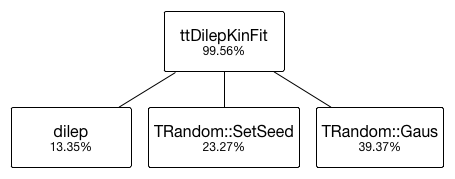
\includegraphics[scale=0.5]{images/prng_256_edited.png}
		\caption{Callgraph subset of the \ttDilepKinFit most time consuming functions for 256 variations per combination.}
		\label{fig:prng256}
	\end{center}
\end{figure}

An analysis of the code showed that the application uses a PRNG available in ROOT, which uses the Mersenne Twister algorithm\cite{MersenneTwister}, resetting the seed for every parameter variation. The Mersenne Twister period is approximately $4.3 * 10^{6001}$, while the maximum amount of pseudo random numbers generated by the application, for the input file used and 1024 variations, is $3 * 10^9$, making the seed reset unnecessary. The removal of this inefficiency granted a 71\% performance improvement.

\subsection{Data Structure Inefficiencies}
\label{data_inef}

Once removed the PRNG seed reset inefficiency, the \ttDilepKinFit still remained the critical region in the application, with no apparent code inefficiency. The most obvious solution is to process in parallel several events from the same input file. However, the function in LipMiniAnalysis that loads events from a file into memory assigns a single global space. This data structure contains information that is modified during the event reconstruction process, and it is overwritten for every event loaded. Changing the data structure to support multiple events in memory simultaneously, and loading all events in the input file at the beginning of the data analysis, would allow the parallel processing of events with low overhead. However, as mentioned in section \ref{problem_and_app} many data analysis applications depend on LipMiniAnalysis preventing any modifications to its structure, so alternative solutions were explored.

\subsection{Alternative Parallel Approaches}

Next step to improve the code execution time is to parallelize \ttDilepKinFit. Note that it is not possible to parallelize the whole event processing since only one is loaded at a time and part of its information is stored in LipMiniAnalysis toolbox. Besides not allowing this parallelization, reading events individually is more inefficient than reading all events at once, where in the former slower random reads are made on the hard drive and in the latter the fast sequential reads are used.

Parallelizing \ttDilepKinFit implies modifying its flow. Currently, for each different combination of jets and leptons from an event, the processed data of each variation of the detector measurements is overwritten. A new data structure is required to hold all combinations of each event. Picking a lepton/jet combination depends on all previous chosen combinations, which serializes the construction of the data structure. Each parallel task (indivisible work segment) selects a combination with variations still to compute, then varies the particles parameters, performs the kinematical reconstruction, and attempts to reconstruct the Higgs boson. A parallel merge is performed after all combinations are computed to get the most accurate reconstruction for the event. Figure \ref{fig:SeqPipeline} presents the sequential and parallel workflow for \ttDilepKinFit.

\begin{figure}[!htp]
	\begin{center}
		\raisebox{-0.5\height}{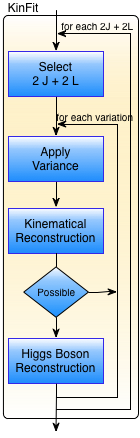
\includegraphics[scale=0.5]{images/sequential_kinfit.png}}
		\raisebox{-0.5\height}{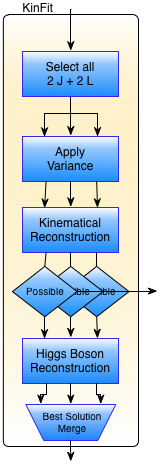
\includegraphics[scale=0.5]{images/parallel_kinfit.png}}
		\caption{Schematic representation of the \ttDilepKinFit workflows: sequential (left) and parallel (right).}
		\label{fig:SeqPipeline}
	\end{center}
\end{figure}

A shared memory parallelization using OpenMP\cite{OpenMP} was devised, as it is the best approach for single shared memory systems. The parallel tasks are grouped into threads, which holds the best reconstruction to minimize the complexity of the merge by reducing through all the threads instead of tasks. The amount of tasks for each thread is balanced dynamically by the OpenMP scheduler, as the workload is irregular since the Higgs boson reconstruction execution is not always computed. Each thread has a private PRNG initialized with different seeds to avoid correlation between the numbers generated.

\begin{figure}[!htp]
	\begin{center}
		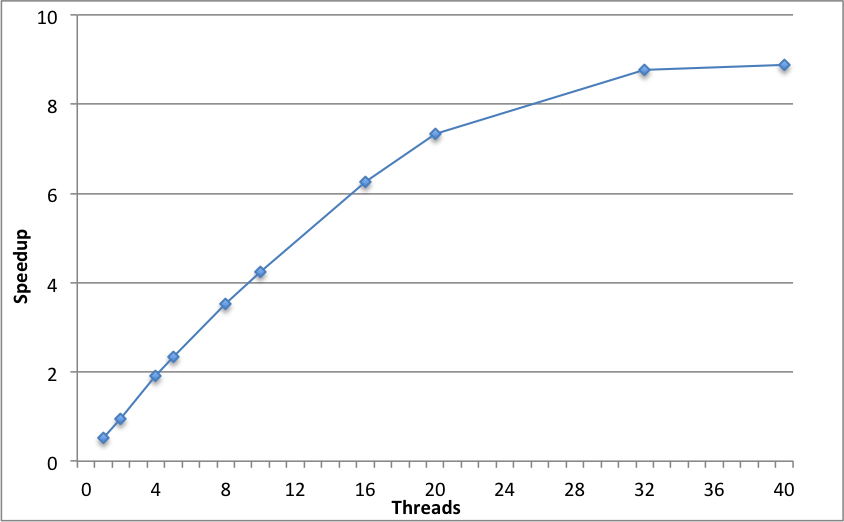
\includegraphics[scale=0.55]{charts/speedup_non_pointer_omp.png}
		\caption{Speedup for the \tth original parallel version of the application.}
		\label{fig:non_pointer_speedup}
	\end{center}
\end{figure}

Figure \ref{fig:non_pointer_speedup} presents the speedups for different number of parallel threads. The purpose of the 1 thread test is to evaluate the parallelization overhead. The best efficient implementation occurs when using 2 and 4 threads, where the application is using almost all resources at each used core. The best overall performance occurs for 40 threads, but it only offers a speedup of 8.8, underusing the available 20 physical cores. Note that there is no significant overhead due to NUMA\footnote{NUMA, Non-Unified Memory Access, since each Xeon device has its own memory controller with attached RAM: RAM access time for each core differs as the RAM is connected to the same device or the neighbour Xeon.} accesses, as seen by the constant increase in performance from 10 to 16 threads. For more than 20 threads all available resources on both CPU devices.

% ------------- pointer version abaixo -----------------

The lack of scalability beyond a low number of parallel threads suggests that inefficiencies may still affect the application, probably caused by the parallelization overhead. Intel's VTune was used to search for hotspots (bottlenecks) on the parallel \tth, since this tool is best suited for profiling parallel applications while providing a user friendly graphic interface. A preliminary analysis showed that the application was spending 20\% of the execution time building the combination data structure for 256 variations.

An analysis of the coded data structure showed that inefficiencies were affecting the performance in specific situations. Data that is read-only on the parallel section is being replicated in each element of the data structure. If the elements were to share a pointer to such data, the overhead of constructing the data structure would be reduced. However, this could lead to worse cache management, due to cache line invalidations, since the application is accessing data on memory more frequently, and the data structuring did not efficiently separate read-only data from read/write data. This is particularly critical in NUMA environments, where communication costs are higher. This was implemented and tested (addressed as \textit{pointer version}), with its speedups ploted in figure \ref{fig:pointer_speedup}. The reference value for the speedup computation is still the same sequential version.

\begin{figure}[!htp]
	\begin{center}
		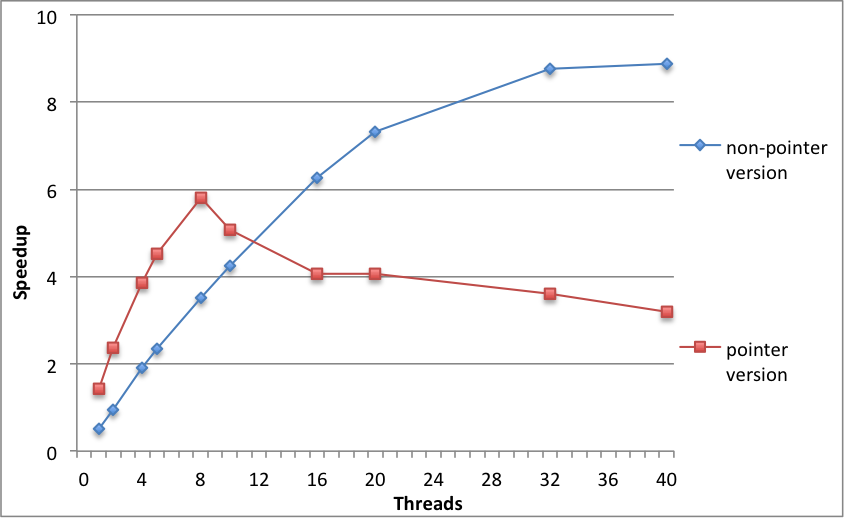
\includegraphics[scale=0.55]{charts/speedup_pointer_omp.png}
		\caption{Speedup for \tth parallel pointer and non-pointer implementations.}
		\label{fig:pointer_speedup}
	\end{center}
\end{figure}

As expected, the best speedup occurs when using only one CPU device. The performance degradation from 8 to 10 threads (on the same device) may be explained by the increase of concurrent accesses to the shared L3 cache. However, this implementation is more efficient than the non-pointer implementation when using only one device. Note that the superlinear speedups is due to the reduction in the data that each thread has to process, making it suitable to be stored in the private L2 cache of each core, avoiding the slower accesses to the L3 cache.
